\documentclass[11pt,reqno]{amsart}

\usepackage{amssymb,mathrsfs,color}
\usepackage{pinlabel}
\usepackage{graphicx}
\usepackage{graphics} 
\usepackage{algorithm}
\usepackage{algorithmic}
\usepackage{natbib}
\usepackage{caption}
\usepackage{tikz}
\usepackage{xspace}


\usetikzlibrary{patterns}


\graphicspath{ {c:/users/mcytrynbaum/documents/rfigures/} {c:/users/mcytrynbaum/Desktop/package/} }
\DeclareGraphicsExtensions{.pdf,.png,.jpg}

\usepackage{amsmath} % for all math functions and operations
\usepackage{amsfonts} % use this to write scripts (e.g. Real nums, etc)
\usepackage{mathtools} %for other math stuff not included in packages above
\usepackage{amsthm} % in case you want the THM: COR: LEMMA: setup
\usepackage[top=1in,bottom=1in,left=1in,right=1in]{geometry} %for setting the margins

%\setlength\parindent{0pt}

\newtheorem{thm}{Theorem}[section]
\newtheorem{lemma}[thm]{Lemma}
\newtheorem{prop}[thm]{Proposition}
\newtheorem{cor}[thm]{Corollary}
\newtheorem{subroutine}[thm]{Subroutine}
\theoremstyle{definition}
\newtheorem{defn}[thm]{Definition}
\newtheorem{examp}[thm]{Example}
\newtheorem{remark}[thm]{Remark}
\setcounter{equation}{0}
\numberwithin{equation}{section}

\renewcommand{\algorithmicrequire}{\textbf{Input:}}
\renewcommand{\algorithmicensure}{\textbf{Output:}}
\newcommand{\prf}{\begin{proof}}
\newcommand{\eprf}{\end{proof}}
\newcommand{\lft}{\left(}
\newcommand{\rt}{\right)}
\newcommand{\be}{\beta}
\newcommand{\eps}{\epsilon}
\newcommand{\wh}{\widehat}
\newcommand{\wt}{\widetilde}
\newcommand{\al}{\alpha}
\newcommand{\bp}{\begin{pmatrix}}
\newcommand{\ep}{\end{pmatrix}}
\newcommand{\inv}{^{-1}}
\newcommand{\var}{\text{Var}}
\newcommand{\cov}{\text{Cov}}
\newcommand{\corr}{\text{Corr}}
\newcommand{\ssumi}{\sum_{i=1}^n}
\newcommand{\ssumj}{\sum_{j=1}^n}
\newcommand{\ssumk}{\sum_{k=1}^n}
\newcommand{\im}{\text{Im}}
\newcommand{\mc}{\mathcal}
\newcommand{\mr}{\mathbb{R}}
\newcommand{\ol}{\overline}
\newcommand{\ul}{\underline}
\newcommand{\prob}{\mathbb{P}}
\newcommand{\ital}{\emph}
\newcommand{\tb}{\textbf}
\newcommand{\pa}{\partial}
\newcommand{\et}{\eta}
\newcommand{\argmax}{\operatornamewithlimits{argmax}}
\newcommand{\lag}{\langle}
\newcommand{\rag}{\rangle}

\newcommand{\pre}{\phi}
\newcommand{\econ}{e}
\newcommand{\coordpre}{\mathrm{CP}}
\newcommand{\prealloc}{(2^X)^A}
\newcommand{\sub}{\subseteq}
\newcommand{\strcore}{\mathrm{C}(X,U)}
\newcommand{\core}{\mathrm{WC}(X,U)}
\newcommand{\stable}{\mathrm{S}(X,U)}
\newcommand{\fecon}{\mathrm{E}}
\newcommand{\fix}{\mathcal{E}}
\newcommand{\suq}{\succeq}
\newcommand{\peq}{\preceq}
\newcommand{\su}{\succ}
\newcommand{\pe}{\prec}
\newcommand{\toppre}{\ol{\pre}}
\newcommand{\bopre}{\ul{\pre}}
\newcommand{\strongc}{\mathcal{G}}
\newcommand{\strongcomp}{S}
\newcommand{\acto}{Q_0} 
\newcommand{\actok}{Q_0^k} 
\newcommand{\actokk}{Q_0^{k+1}} 
\newcommand{\actot}{Q_0^t} 
\newcommand{\actott}{Q_0^{t+1}} 
\newcommand{\actol}{Q_0^{\ell}} 
\newcommand{\actoll}{Q_0^{\ell + 1}} 
\newcommand{\acta}{Q_A} 
\newcommand{\actak}{Q_A^k} 
\newcommand{\actakk}{Q_A^{k + 1}} 
\newcommand{\actc}{Q_I} 
\newcommand{\actck}{Q_I^k} 
\newcommand{\actckk}{Q_I^{k + 1}} 
\newcommand{\actat}{Q_A^t} 
\newcommand{\actatt}{Q_A^{t + 1}} 
\newcommand{\actct}{Q_I^t} 
\newcommand{\actctt}{Q_I^{t + 1}} 
\newcommand{\act}{Q} 
\newcommand{\actt}{Q_{temp}} 
\newcommand{\actacum}{\wh{Q_A}} 
\newcommand{\actocum}{\wh{Q_0}} 
\newcommand{\disto}{d}
\newcommand{\distt}{D}
\newcommand{\preo}{\pre^{0}} 
\newcommand{\pren}{\pre_{0}} 
\newcommand{\pref}{\pre^{f}} 
\newcommand{\coll}{I}
\newcommand{\collk}{I^k}
\newcommand{\res}{\act_{int}}
\newcommand{\reach}{H}
\newcommand{\forest}{F}
\newcommand{\fixfind}{\mathcal{E}_C}
\newcommand{\fixfindk}{\mathcal{E}^k_C}
\newcommand{\fixfindkk}{\mathcal{E}^{k + 1}_C}
\newcommand{\fixtemp}{\mathcal{E}_{temp}}
\newcommand{\fixtempk}{\mathcal{E}^k_{temp}}
\newcommand{\fixtempkk}{\mathcal{E}^{k + 1}_{temp}}
\newcommand{\fixtempt}{\mathcal{E}^t_{temp}}
\newcommand{\fixtemptt}{\mathcal{E}^{t + 1}_{temp}}
\newcommand{\stp}{\mathrm{STOP}}
\newcommand{\pair}{(F,I)}
\newcommand{\roott}{R}
\newcommand{\depth}{D}
\newcommand{\unproc}{\mathcal{J}_u}
\newcommand{\glob}{G}
\newcommand{\optwo}{T_2}
\newcommand{\opthree}{T_3}
\newcommand{\oper}{F}
\newcommand{\point}{P}
\newcommand{\lattice}{L}

\newcommand{\topx}{\ol{X}}
\newcommand{\topy}{\ol{Y}}
\newcommand{\botx}{\ul{X}}
\newcommand{\boty}{\ul{Y}}
\newcommand{\pairi}{(X_i,Y_i)}
\newcommand{\pairj}{(X_j,Y_j)}
\newcommand{\pairp}{(X',Y')}
\newcommand{\pairpp}{(X'',Y'')}

%%%% ALGORITHM CONTROLS
\newcommand{\infcombiniti}{(i)\xspace}
\newcommand{\infcombinitii}{(ii)\xspace}
\newcommand{\infcombinitiii}{(iii)\xspace}
\newcommand{\infcombgraphi}{(1)\xspace}
\newcommand{\infcombgraphii}{(2)\xspace}
\newcommand{\infcombgraphiii}{(3)\xspace}
\newcommand{\infcombcomba}{(a)\xspace}
\newcommand{\infcombcombb}{(b)\xspace}

\newcommand{\infacredi}{(i)\xspace}
\newcommand{\infacredii}{(ii)\xspace}
\newcommand{\infacbstopa}{(a)\xspace}
\newcommand{\infacbstopb}{(b)\xspace}
\newcommand{\infacstoptwi}{(i)\xspace}
\newcommand{\infacstoptwii}{(ii)\xspace}
\newcommand{\infacstoptwiii}{(iii)\xspace}
\newcommand{\infacstoptha}{(a)\xspace}
\newcommand{\infacstopthb}{(b)\xspace}
%%%%

\date{Novemeber 21, 2015}
\title{Using Lattice Geometry to Find All Stable Allocations}
\author{Max Cytrynbaum} 
\thanks{I am very grateful to Scott Kominers for continual guidance and for providing the inspiration for this project. This project was completed with the help of an Economic Design Summer Fellowship from the Harvard Society of Fellows. Please send comments and suggestions to mcytrynbaum@gmail.com.}

\begin{document}
\maketitle
\begin{abstract}
In this paper, we give an algorithm to find all core allocations in a highly general model of multilateral many-to-many matching with contracts.
We develop a notion of information sharing in lattices, showing how lattice geometry and information sharing can be exploited to produce a relatively fast algorithm that returns the full list of core outcomes.
We show how to apply this technique to more general economic problems and, as an application, construct the first algorithm to find \emph{all} stable allocations in bilateral matching with contracts when agents have substitutable preferences. 
\end{abstract}

\section{Introduction}
\subsection{Introduction and Motivation}
This paper extends an algorithm pioneered in \cite{EcheniqueYenmez2013} to find \emph{all} core allocations in a general model of multilateral many-to-many matching with contracts.
Our model nests a large number of previously considered matching models.
We show that, as in the case of matching with preferences over colleagues in \cite{EcheniqueYenmez2013}, core allocations can be characterized in terms of the fixed points of an antitone operator on a certain complete lattice.
Our main contribution is to show how to fully exploit the geometric relationships implied by the problem's lattice structure.
We develop a notion of information sharing in lattices, construct and prove correctness for an algorithm that implements this idea, and show how this approach may be extended to a wider class of economic problems for which there is a complete lattice structure. 
To conclude, we restrict our attention to two-sided many-to-many matching with contracts with substitutable preferences, showing how information sharing may be used to find \emph{all} stable allocations.

There are a variety of results showing the existence of a lattice of stable outcomes when preferences satisfy a substitutability condition.
Usually, these results proceed by showing that substitutability implies the existence of an isotone operator on a complete lattice containing the stable matchings\footnote{See, for instance, \cite{HatfieldMilgrom2005} or \cite{HatfieldKominers2010}.}.
By iteration from a maximal element, one eventually arrives at an extremal stable matching.
Conversely, in the absence of substitutability, not only are stable matchings not guaranteed to exist, but the usual isotone operator is not guaranteed to find any that do exist.
Even if substitutability does hold, it is often unclear how to find any but the extremal stable matchings.

This paper aims to address some of these issues.
The core is a natural replacement for stability in the absence of substitutability guarantees; indeed, in many classical models, such as the marriage problem, the core coincides with the set of stable matchings\footnote{\cite{RothSotomayor1990}.}. 
We show that, even without a substitutability guarantee, in which case the usual operator for finding stable matchings is not necessarily isotone, there still exists a relatively fast algorithm that returns all \emph{core} allocations or shows that none exist. 
When substitutability does hold, we show how our technique can be modified to find \emph{all} stable matchings, not just the extremal ones.

As noted by \cite{KlausKlijn2005}, substitutability is an unreastically stringent condition in many real world markets.
Thus, our algorithm has practical value for a market designer interested in finding reasonable economic outcomes in such markets.

Lattice structures arise frequently in economics.
We show how lattice geometry can be combined with economic problem structure to develop a notion of information sharing in lattices that allows for faster computation of objects of economic interest.  
The algorithm developed in this paper thus has independent economic value outside of matching theory. 

\subsection{Related Literature}
Omitted for this writing sample.

\section{Characterizing Core Allocations} \label{section:strcore}
In this section, we show how core allocations can be characterized as the fixed points of an antitone operator on a certain complete lattice.
First, we give details on our model and notation.

\subsection{Model and Solution Concepts}
We consider a finite set of contracts $X$, each of which is associated with at least one agent $a\in A$. 
We call a subset $Y\sub X$ an \emph{allocation}, and let $2^X$ denote the set of all allocations. 
Let $d(x)$ be the set agents associated with a contract $x\in X$, and extend this definition to allocations by writing $d(Y) \equiv \bigcup_{y\in Y} d(y)$.
Note that, in general, we may have $|d(x)| > 2$ for multilateral contracts.
For instance, we can view $X$ as the set of potential multilateral relationships in a trading network\footnote{This setting is thus a slight generalization of \cite{HatfieldKominers2010} model of bilateral contracts in a trading network.}. 
In particular, we \emph{do not} impose a two-sided market structure in this section.

For $a\in A$, we let $Y_a = \{y\in Y: \, a\in d(y)\}$ denote the set of contracts associated with that agent (note that we may have $Y_a = \emptyset$). Thus, $2^{X_a}$ denotes the set of all allocations naming an agent $a\in A$. 
We assume that each $a\in A$ has strict preferences over $Y \in 2^{X_a}$, where the utility of an allocation is given by the one-to-one function $U_a: 2^{X_a} \to \mr$.
Let $\su_a$ denote the strict preference relation induced by these utility functions over bundles $Y \in 2^{X_a}$, with $\suq_a$ denoting the weak relation. Thus, $Y \suq_a  Z \iff$ $Y \su_a Z$ or $Y = Z$.
Throughout this paper, we will assume that $\emptyset_a \in X$ for all $a \in A$, where $\emptyset_a$ denotes $a$ being unmatched. Note that $d(\emptyset_a) = \{a\}$. 

An allocation $Y \sub X$ is said to be in the \emph{core}\footnote{The core concept defined here is sometimes also called the strong core or ``core by weak domination''; see \cite{RothSotomayor1996}, for instance.
Here, we follow the core concept used in \cite{EcheniqueYenmez2013}.}
if there does not exist a non-empty blocking set $Z \sub X$ such that 
\[
U_b(Z_b) \geq U_b(Y_b) \qquad  \forall b\in d(Z)
\]
where \emph{at least one} of the above inequalities holds strictly.
We denote the core by $\strcore$. 

Similarly, an allocation $Y$ is said to be in the \emph{weak core} if there does not exist a non-empty blocking set $Z \sub X$ such that 
\[
U_b(Z_b) > U_b(Y_b) \qquad  \forall b\in d(Z)
\]
We denote the weak core by $\core$. 
Note that $\core \supseteq \strcore$.

It is easy to see that core allocations need not exist in such a general setting.
Our approach will be to construct an algorithm that either finds all core allocations or shows that none exist. 

\subsection{Fixed Preallocations and the Core}
We build an appropriate framework in which to generalize the fixed point construction discussed above. 
We start by generalizing the classical notion of a \emph{prematching}. 

\begin{defn}[Preallocation] We call a map $\pre: A \to 2^X$ a \emph{preallocation} if $\pre(a) \in 2^{X_a}$ for all $a\in A$. Let $(2^X)^A$ denote the set of all preallocations.  
\end{defn}

Intuitively, a preallocation assigns each agent to a bundle of contracts naming him or her. We may think of $\pre(a)$ as the set of contracts ``held'' by agent $a$.   

We can associate each allocation $Y\subseteq X$ with a unique preallocation $\pre_Y$ in a natural way by setting $\pre_Y(a) = Y_a$ for $a \in d(Y)$ and $\pre_Y(a) = \emptyset_a$ otherwise.
\begin{remark} Note, however, that not all preallocations can be derived from allocations in this way.
For example, consider the case where $\emptyset \not = \pre(a)_b \not = \pre(b)_a$. In the preallocation $\pre$, $a$ holds contracts naming $b$ that are \emph{not} in the bundle of contracts held by $b$ naming $a$.  
In particular, there does not exist an allocation $Y$ such that $\pre = \pre_Y$. 
\end{remark}

With this example in mind, we say that $\pre \in \prealloc$ is a \emph{coordinated} preallocation if there exists an allocation $Y$ such that $\pre = \pre_Y$. 
We denote the set of all cooordinated preallocations by $\coordpre\sub \prealloc$.
Our method proceeds by identifying allocations $Y \in \strcore$ with fixed points of an operator on preallocations, generalizing the construction in \cite{EcheniqueYenmez2013}.

For each agent $a \in A$, we define 

\[
V(\pre, a) = \{Z \in 2^{X_a}: \exists Y \in 2^X \, s.t. \,  Y_a = Z, \, Y_b \suq_b \pre(b) \: \forall b \in d(Y)\setminus\{a\} \}
\]

Intuitively, $V(\pre, a)$ is the \emph{possibility set} for an agent $a$ at a preallocation $\pre$. 
It contains all bundles of contracts naming $a$ that are part of a larger economy $Y$ in which every other agent $b \in d(Y)$ weakly prefers their contracts under $Y$ to their contracts under the preallocation $\pre$.  

Next, we define an operator $T: \prealloc \to \prealloc$ by setting $T \pre(a) = \max V(\pre, a)$, where the maximum is taken under the preference relation $\suq_a$ for each $a \in A$.
Note that $\emptyset_a \in V(\pre,a)$ for any $\pre \in \prealloc$, so $T$ is well-defined. Let $\fix(T)$ denote the fixed points of $T$. Define $\fecon(T) = \{Y \in 2^X: \, \pre_Y \in \fix(T)\}$, the collection of allocations $Y$ whose corresponding preallocation $\pre_Y$ is fixed by $T$.

Before our first result, we note a simple fact: if $\pre \in \coordpre$, then $\pre(a) \in V(\pre, a)$.
To see this, note that $\pre \in \coordpre$ means that there exists $Y \sub X$ with $\pre = \pre_Y$. 
Then $Y$ is an allocation satisfying the conditions in $V(\pre_Y,a)$, so that $Y_a  = \pre(a) \in V(\pre,a)$. 
With the definitions above, we have a simple result
\begin{lemma} \label{lemma:strictcore}
$\fecon(T) = \strcore$
\end{lemma}
\prf
First, suppose that $Y \not \in \strcore$. Then by definition, there exists some blocking allocation $\emptyset \not = Z \sub X$ such $Z_b \suq_b Y_b$ for all $b \in d(Z)$.
Let $a \in d(Z)$ be such that the inequality above is strict, and consider $\pre = \pre_Y$. 
In particular, $Z_b \suq_b \pre_Y(b)$ for all $b \in d(Z) \setminus \{a\}$, so that $Z_a \in V(\pre_Y, a)$.
Then $T \pre_Y(a) = \max V(\pre_Y, a) \suq_a Z_a \su_a Y_a = \pre_Y(a)$, so $T\pre_Y(a) \not = \pre_Y(a)$, and $Y \not \in \fecon(T)$.  

Suppose, conversely, that $Y \not \in \fecon(T)$ so that $\pre_Y \not \in \fix(T)$.  
Then there exists an agent $a \in A$ such that $T\pre_Y(a) = Z_a \not = \pre_Y(a)$ for some allocation $Z$.  
By the definition of $V(\pre_Y,a)$, we have $Z_b \suq_b \pre_Y(b) = Y_b$ for $b \in d(Z) \setminus \{a\}$.
We know $\pre_Y$ is coordinated, so by the simple fact above $\pre_Y(a) \in V(\pre_Y,a)$.
Then $Z_a = T \pre_Y(a) \su_a \pre_Y(a) =  Y_a$. Then $Z$ is a blocking coalition for $Y$, so $Y \not \in \strcore$.  
\eprf
Thus, we have identified $\strcore$ with the set of \emph{coordinated} preallocations $\pre \in \coordpre$ such that $T \pre = \pre$. 
This result shows that an algorithm that finds all $\pre \in \fix(T)$ will also find all core matchings. 

However, if there are \emph{uncoordinated} preallocations that are also fixed by $T$, such an algorithm may return extraneous solutions not associated with any core matching.
The following lemma, which is essential for the construction of our algorithm, shows that there are no such preallocations.
Note that this result significantly generalizes the corresponding lemma in \cite{EcheniqueYenmez2013} and also subsumes the main result of \cite{Kojima2007b}. 

\begin{lemma} \label{lemma:coordinated}
$\fix(T) \sub \coordpre$
\end{lemma}
\prf
We begin with an important fact that will be used repeatedly.
Suppose that $\pre \in \fix(T)$. Then for any $a \in A$, we have $\pre(a) = T\pre(a) \in V(\pre,a)$.
Thus, there exists an allocation $Y$ such that $Y_a = \pre(a)$, and $Y_b \suq_b \pre(b)$ for all $b \in d(Y) \setminus \{a\}$.
Since $Y_a = \pre(a)$, then in fact $Y_b \suq_b \pre(b)$ holds \emph{for all} agents $b \in d(Y)$. 
For any $b \in d(Y)$, $Y$ then satisfies the conditions in the definition of $V(\pre,b)$, so $Y_b \in V(\pre,b)$. 
Therefore, $\pre(b) = T\pre(b) \suq Y_b \suq \pre(b)$, so equality holds throughout. In particular, $Y_b = \pre(b)$ for all $b \in d(Y)$. 

Fix $a_1 \in A$. Since $\pre \in \fix(T)$, the argument above shows that there exists an allocation $Y$ such that $Y_{a_1} = \pre(a_1)$, and, in particular, $Y_b = \pre(b)$ for all $b \in d(Y)$. 
Therefore, the collection of global allocations available to $a_1$ at $\pre$ 
\[\glob(\pre,a_1) = \{Y \in 2^X: Y_{a_1} = \pre(a_1), \: Y_b \suq \pre(b)\: \forall b \in d(Y)\}\]
is non-empty, so there exists an allocation 

\[
Y \in \argmax_{Z \in \glob(\pre,a_1)} |d(Z)|
\]

Let $A_1 = d(Y)$. If $A_1 = A$, we are done, since then by the construction above $Y_a = \pre(a)$ for all $a \in A$, so $\pre = \pre_Y$ and $\pre \in \coordpre$. 

Then assume that $A_1 \not = A$, and pick $a_2 \in A \setminus A_1$. By the fact at the beginning of the proof, there exists an allocation $Z$ such that $Z_{a_2} = \pre(a_2)$, and, in fact, $\pre(b) = Z_b$ for all $b \in d(Z)$. 
Define $A_2 = d(Z) \cap A_1^c$, which is non-empty by construction.
Let $b \in A_2$. We will show that $d(\pre(b)) \cap A_1 = \emptyset$.
That is, under the preallocation $\pre$, agent $b \in A_2$ is \emph{not} holding any contracts that name agents in $A_1$. 

Suppose not, so there exists $c \in A_1 \cap d(\pre(b))$.
Then, in particular, $c \in d(\pre(b)) = d(Z_b) \sub d(Z)$, so applying the fact proved at the beginning, $Z_c = \pre(c) = Y_c$. 
Since $c \in d(Z_b)$, there exists a contract $z \in Z_c$ naming both $c$ and $b$.
Then $b \in Z_c = Y_c$, so $b \in d(Y_c) \sub d(Y) = A_1$, so $b \in A_1 \cap A_2 = \emptyset$. 
This is a contradiction, so it must be the case that $d(\pre(b)) \cap A_1 = \emptyset$ for all $b \in A_2$. 

Define $S = \bigcup_{b \in A_2} \pre(b)$. We have just shown that $d(S) \sub A_1^c$.
We also have $d(S) = \bigcup_{b \in A_2} d(\pre(b)) = \bigcup_{b \in A_2} d(Z_b) \sub d(Z)$, so $d(S) \sub A_1^c \cap d(Z) = A_2$.
Clearly $b \in d(\pre(b))$ for all $b \in A_2$, so $A_2 \sub d(S)$. Then $A_2 = d(S)$. 

Set $W = Y \cup S$. We have now shown that $A_2 \not = \emptyset$ and $A_1 \cap A_2 = \emptyset$.
Since $d(Y) = A_1$ and $d(W) = A_2$, it follows that $W \cap Y = \emptyset$, so we have  

\begin{enumerate}
\item $W_b = Y_b = \pre(b)$ for all $b \in A_1$.
\item $W_b = S_b = \pre(b)$ for all $b \in A_2$.
\end{enumerate}

Then apparently $W \in \glob(\pre,a_1)$ as defined above. However, by construction $|d(W)| > |d(Y)|$, which contradicts our original choice of $Y$.
This finishes the proof.
\eprf
\subsubsection{Discussion}
Combining these lemmas, we see that searching for core allocations in a very general model of multilateral matching with contracts is equivalent to searching for the fixed points of $T$. 
Our algorithm depends heavily on this result, which shows, critically, that the fixed points $\fix(T)$ are only as dense in $\prealloc$ as the core outcomes.

Our maximal domain results will show that this is not the case for the natural extension of this method to \emph{weak} core outcomes $\core$.
For weak core outcomes, where the lattice algorithm fails, $T$ also fixes at a large number of extraneous, uncoordinated preallocations (see Lemma~\ref{lemma:core}). 

\subsection{The Lattice of Fixed Preallocations}
In this section, we generalize constructions from \cite{EcheniqueYenmez2013} showing the the fixed points of the squared operator $T^2$ form a lattice. 
First, we define a natural partial order on the set of preallocations $\prealloc$.

Say that $\pre \su \pre'$ if and only if $\pre(a) \suq_a \pre'(a)$ for all $a \in A$, where at least one of these inequalities \emph{holds strictly}. 
Thus, we write $\pre \suq \pre'$ if and only if $\pre \su \pre'$ or $\pre = \pre'$. 
This is a product order on a product space, which makes $\prealloc$ into a complete lattice. 
Next, we give a sequence of results concerning the operator $T$ and its fixed points. 
These results are an almost direct extension of the results in Lemma 4 through Proposition 8 of \cite{EcheniqueYenmez2013}.
For the purposes of illustration, we include the proof the first result for the more general framework of preallocations considered in this paper.
The rest of the lemmas follow from straightforward extensions of the work in \cite{EcheniqueYenmez2013}. 
\begin{lemma} \label{lemma:antitone}
$T$ is antitone 
\end{lemma}
\prf
Let $\pre \peq \pre'$ be preallocations.
Fix $a \in A$, and let $Z \in V(\pre',a)$.
Then there is an allocation $Y \sub X$ with $Y_a = Z$ such that $Y_b \suq_b \pre'(b)$ for $b \in d(Y) \setminus \{a\}$.
Then $Y_b \suq_b \pre'(b) \suq_b \pre_b$ also for all such agents, so we also have $Z \in V(\pre,a)$.
Then $V(\pre,a) \supseteq V(\pre',a)$, so that $T\pre(a) \suq T\pre'(a)$. The agent $a$ was arbitrary, so $T\pre \suq T\pre'$ under our partial order. 
\eprf
The following lemmas follow exactly as in \cite{EcheniqueYenmez2013}, using the antitonicity of $T$. 
\begin{cor} $T^2$ is isotone, and $\fix(T^2)$ is a non-empty complete lattice. 
\end{cor}
\begin{lemma} \label{lemma:order}
No two preallocations $\pre$ and $\pre'$ can be compared under the partial order on $\prealloc$.
\end{lemma}
\begin{lemma} \label{lemma:top}
There exist preallocations $\ol{\pre}$ and $\ul{\pre}$ such that for all $\pre \in \fix(T)$, we have $\ol{\pre} \suq \pre \suq \ul{\pre}$. Moreover, if $\pre = \ol{\pre}$ or $\pre = \ul{\pre}$, then $\fix(T) = \{\pre\}$. 
\end{lemma}

\section{Sharing Lattice Information to Find All Core Allocations}
\subsection{Introduction}
In this section, we give an algorithm that finds \emph{all} core allocations in the model of multilateral matching with contracts considered above.
Our algorithm builds upon the original approach in \cite{EcheniqueYenmez2013}.
In particular, we show how to fully exploit the problem's complete lattice structure to more efficiently find the full set of core matchings. 

The algorithm proceeds by successively initializing modified versions of the original matching problem, in which each agent has a truncated preference list.
Our main contribution is to realize that many of the subproblems created while searching the lattice $\fix(T^2)$ share geometric information with other subproblems.
We show how fast digraph algorithms may be used to combine this shared information and more quickly identify the full set of core matchings. 

\subsection{Intuition and Notation} \label{section:description1}
\subsubsection{Algorithm Intuition}
Let $\pre^*$ denote the largest preallocation under the partial order $\su$.
That is, $\pre^*(a) = \argmax U_a(\pre(a))$ for each $a \in A$.
Suppose that the total number of agents $|A| = m > 0$.
We will use $\langle \pre \rangle$ or $\langle \pre(1) \hdots \pre(m) \rangle$  to denote a version of the original problem in which each agent $a$'s preference list is truncated to allocations in $2^{X_a}$ ranked weakly below $\pre(a)$ by agent $a$. 
We will often identify a problem $\lag \pre \rag$ with its maximal point $\pre$.
Let $\fix(\pre) \equiv \{\pre' \in \fix(T): \: \pre' \peq \pre\}$ denote the fixed points of $T$ below $\pre$.  

By Tarski's Theorem\footnote{This is easy to see.
Note that $T^2 \pre^* \peq \pre^*$ by maximality, so $(T^2)^k \pre^* \peq (T^2)^{k+1} \pre^*$ for any $k\geq 1$ by isotonicity.
Then this sequence is monotonically decreasing and bounded above $\min \fix(T^2)$ on a finite lattice, so it converges in finitely many iterations, say at $k = \ell$.
Let $\pre' \in \fix(T^2)$ another fixed point, then $\pre^* \suq \pre'$, so $\toppre = (T^2)^{\ell} \pre^* \suq (T^2)^{\ell} \pre' = \pre'$, so $\toppre = \max(\fix(T^2))$.}, the sequence $(T^2)^k \pre^*$ converges to a preallocation $\toppre$, fixed by $T^2$, which is the maximal point of the lattice $\fix(T^2)$.
If $T \toppre = \toppre$, then by Lemma~\ref{lemma:top} showing that no elements of $\fix(T^2)$ are ranked by ``$\peq$'', $\fix(T) = \{\toppre\}$.
So suppose that $T \toppre \not = \toppre$. 
Clearly $\fix(T) \sub \fix(T^2)$ for any operator, and, by iteratively applying $T^2$, we have learned that $\fix(T) \sub \fix (T^2) \sub \{\pre': \pre' \peq \toppre\} \equiv \{\pre' \peq \toppre\}$.
We will sometimes denote relations of this type by $\fix(T) \peq \toppre$. 

Since $T\toppre \not = \toppre$, apparently $\fix(T) \sub \bigcup_{i = 1}^m \{\pre' \peq \toppre - e_i\}$, where $e_i$ denotes the standard unit vector\footnote{identifying $\prealloc$ with a grid in $\mr^m$ as above.} in $\mr^m$. 
Consider a subproblem of the form $\lag \toppre - e_i \rag$, and let $T_i$ be the operator corresponding to this subproblem, where agents' preferences are truncated above $\toppre - e_i$.
The key insight of \cite{Echenique2007Equilibria}, which generalizes to the current model, is that $\fix(T) \cap \{\pre' \leq \toppre - e_i\} \sub \fix(T_i)$.
That is, the fixed points of $T$ contained in the cone $\{\pre' \peq \toppre - e_i\}$ are also fixed points of the new problem $\lag \toppre - e_i \rag$ with operator $T_i$. 
Then apparently we have $\fix(T) \cap \{\pre' \leq \toppre - e_i\} \sub \fix(T_i) \sub \fix(T_i^2)$, so information about the lattice of fixed points of $T_i^2$ can be used to bound $\fix(T)$.
The general result in our setting is as follows 
\begin{lemma} \label{lemma:contain}
Suppose $\pre \peq \wh{\pre}$, and let $\wh{T}$ denote the core operator for the problem $\lag \wh{\pre} \rag$.
If $\pre \in \fix(T)$, then $\pre \in \fix(\wh{T})$.
In particular, $\fix(T) \cap \{\pre \leq \wh{\pre}\} \sub \fix(\wh{T}^2)$. 
\end{lemma}
\prf
Let $\wh{V}(\pre, a)$ be the defining set for $\wh{T}$ in the subproblem.
Then for any $a \in A$ and $\pre \in \prealloc$ we have 
$\wh{V}(\pre,a)  = \{Z \in 2^{X_a}: \exists Y \in 2^X \, s.t. \,  Y_a = Z, \, \wh{\pre}(b) \suq_b Y_b \suq_b \pre(b) \: \forall b \in d(Y)\setminus\{a\} \}$
then clearly $\wh{V}(\pre,a) \sub V(\pre,a)$.  
We can compute $\wh{T}\pre(a) = \max \wh{V}(\pre,a) \leq \max V(\pre,a) = T\pre(a)$ for any preallocation $\pre$. 

Now, suppose that $\pre \in \fix(T)\cap\{\pre' \peq \wh{\pre}\}$.
Then we have have $\pre(a) = T\pre(a) \suq_a \wh{T}\pre(a)$ for all $a \in A$. 
By Lemma~\ref{lemma:coordinated} above, $\fix(T) \sub \coordpre$, so $\pre = \pre_Y$ for some allocation $Y \in 2^X$.
In particular, $Y_a = \pre(a) \peq_a \wh{\pre}(a)$, so $\pre(a) \in \wh{V}(\pre,a)$.
Then by the definition of $\wh{T}$, we get $\wh{T}\pre(a) \suq_a \pre(a)$. 

Combining this with the statement above, we have $\pre(a) = \wh{T} \pre(a)$, so $\pre \in \fix(\wh{T})$. 
\eprf 
Returning to the discussion above, we showed that $\fix(T) \sub \bigcup_{i = 1}^m \{\pre' \peq \toppre - e_i\}$, a union of cones in the lattice of preallocations. 
That is, $\fix(T) \sub \bigcup_{i = 1}^m \fix(\toppre - e_i)$.
Fix $i$ and consider $\fix(\toppre - e_i)$, the fixed points of $T$ below $\toppre - e_i$.
For convenience, denote $S_i \equiv T_i^2$ and $\toppre_i \equiv \toppre - e_i$.
Starting with $\toppre_i$, the unanimously most preferred preallocation in the subproblem $\lag \toppre_i \rag$, Lemma~\ref{lemma:strictcore} and the Tarski argument used above show that each iteration of $S_i$ gives a ``cone guarantee'' on the fixed points $\fix(T)$ of the form $\fix(\toppre_i) \peq S_i^k \toppre_i$.

Pursuing this strategy for $i = 1 \hdots m$, we can bound the complete set of fixed points $\fix(T)$ in a union of subproblem cones. 
We continue this strategy recursively by generating $m$ new subproblems whenever a monotonic sequence of the form $S_i^k \toppre_i $ stops at a fixed point of $S_i^k$. 
In this way, we will eventually find the full set of core outcomes, directly extending the \cite{EcheniqueYenmez2013} algorithm to the present setting.  

However, depending on the structure of the lattice $\fix(T^2)$, the strategy described above can actually be quite similar to greedy search.  
In particular, the number of subproblems generated at the kth recursive level scales exponentially in $k$ as $|A|^k$.As we will show, many of the subproblems generated by this strategy are either redundant or do not need to be solved completely.
We will show that we can capitalize on the structure of the preallocation lattice by allowing subproblems to share geometric information with each other. 
With this modification, evaluation of the full Tarski sequence $S_i^k \toppre_i$ is often unnecessary. 
In fact, it is often the case that subproblems can be stopped or removed entirely after a few iterations. 
We will illustrate this idea with a couple of simple examples.  

\subsubsection{Example 1 - Colliding Subproblem Cones}
In this section, we give a simple example of how subproblems can share information.
For easy of visualization, consider the case $|A| = 2$. As noted previously, we may identify $\prealloc$ with a grid, in this case in $\mr^2$.
As above, we iterate $T^2$ to find $\toppre = \max \fix(T^2)$, which we identify, for instance, with the integer lattice point $(10,10) = \toppre$. 
Using the notation above, there are isotone operators $S_1 = T_1^2$ and $S_2 = T_2^2$ corresponding to the subproblems $\lag \toppre - e_1 \rag$ and $\lag \toppre - e_2 \rag$, respectively. 

Beginning with subproblem 1, suppose that $S_1 (9,10) = (8,10)$, $S_1^2 (9,10) = (7,9)$, and $S_1^3 (9,10) = (7,9)$.
By our arguments above, we now have a cone guarantee on the fixed points in the first subproblem; specifically, $\fix(T) \cap \{(x,y) \peq (9,10)\} \peq (7,9) \peq (10,9) = \toppre_2$.
Therefore, $\fix(\toppre_1) = \fix(T) \cap \{(x,y) \peq (9,10)\} \sub \fix(T) \cap \{(x,y) \peq (10,9)\} = \fix(\toppre_2)$. 
That is, the solutions to subproblem 1, the fixed points of $T$ in $\{(x,y) \peq (9,10)\}$, are \emph{contained} in the set of solutions to subproblem 2. 

Now suppose that we stop working on subproblem 1 and begin iterating with $S_2$.
Suppose that $S_2(10,9) = (10,6) = S_2^2(10,9)$, so the sequence stops.
Then we have learned that $\fix(\toppre_1) \sub \fix(\toppre_2) \peq (10,6)$. 
However, by iterating $S_1$, we also learned that $\fix(\toppre_1) \peq (7,9)$. 
Then apparently $\fix(\toppre_1)$ is contained in the cone intersection $\{(x,y) \peq (7,9)\} \cap \{(x,y) \peq (10, 6)\} = \{(x,y) \peq (7,6) \}$. 
That is, by \emph{combining the information} from subproblem 2 with subproblem 1, we have learned that $\fix(\toppre_1) \peq (7,6)$. 

\begin{figure} \label{fig:rectangles}
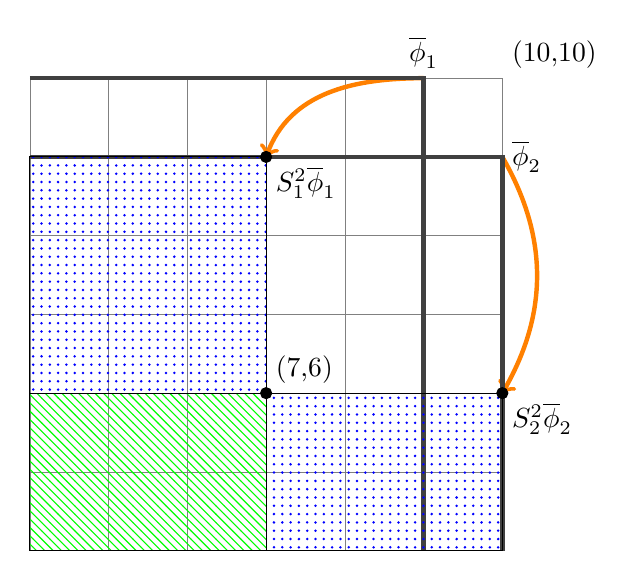
\begin{tikzpicture}
\draw[help lines] (0,0) grid (6,6);
%\draw[fill] (5,6) circle [radius=0.05];
%\draw[fill] (6,5) circle [radius=0.05];
\draw[orange,->, ultra thick] (5,6) to [out=180, in=70] (3,5);
\draw[orange,->, ultra thick, bend left] (6,5) to (6,2);
\draw[darkgray, ultra thick] (0,6) -- (5,6) -- (5,0);
\draw[darkgray, ultra thick] (0,5) -- (6,5) -- (6,0);
\draw[blue] (0,5) -- (3,5) -- (3,0);
\draw[blue] (0,2) -- (6,2) -- (6,0);
\draw[pattern = dots, pattern color = blue] (0,5) rectangle (3,2);
\draw[pattern = dots, pattern color = blue] (3,0) rectangle (6,2);
\draw[pattern = north west lines, pattern color = green] (0,0) rectangle (3,2);
\node[above right] at (6,6) {(10,10)};
\node[above right] at (3,2) {(7,6)};
\node[above] at (5,6) {$\toppre_1$};
\node[right] at (6,5) {$\toppre_2$};
\node[below right] at (3,5) {$S_1^2 \toppre_1$};
\node[below right] at (6,2) {$S_2^2 \toppre_2$};
\draw[fill] (3,2) circle [radius=0.07];
\draw[fill] (3,5) circle [radius=0.07];
\draw[fill] (6,2) circle [radius=0.07];
\end{tikzpicture}
\caption{Combining Information from Subproblem Cones Guarantees}
\end{figure}

Note that, even if we learn $\fix(\toppre_1) \sub \fix(\toppre_2)$, we may still wish to retain the information associated with subproblem 1. 
If, for instance, the outcome for subbproblem 2 was instead that $S_2(10,9) =  (9,6) = S_2^2(10,9)$, then we would also know that $\fix(\toppre_2) \sub \fix(\toppre_1)$, so that $\fix(\toppre_2) \peq \min((9,6),(7,9)) = (7,6)$ and, in fact, $\fix(\toppre_1) = \fix(\toppre_2)$.
The idea of equivalent subproblems is explored further in the next example. 

\subsubsection{Example 2 - Chutes and Ladders}
In this section, we give intuition for how to efficiently combine information and track the relations between different subproblem cones. 
Consider the case $|A| = 3$, where we identify $(10,10,10) = \toppre = \max \fix(T)$. 
After initializing subproblems at $(9,10,10)$, $(10,9,10)$ and $(10,10,9)$, suppose that we find $S_1(9,10,10) = (9,8,10)$, $S_2(10,9,10) = (10,9,7)$, and $S_3(10,10,9) = (9,10,9)$. 
As argued above, this shows that $\fix(\toppre_1) \peq (9,8,10) \peq (10,9,10) = \toppre_2$, so that $\fix(\toppre_1) \sub \fix(\toppre_2)$. 
Similarly, our calculations with $S_2$ and $S_3$ show that $\fix(\toppre_2) \sub \fix(\toppre_3)$ and $\fix(\toppre_3) \sub \fix(\toppre_1)$. 
Combining all these relations, apparently $\fix(\toppre_1) = \fix(\toppre_2) = \fix(\toppre_3) \peq (9,8,7)$, so the subproblems are equivalent.  
Thus, we can collapse all of these subproblems to a new subproblem started at $\pre' = (9,8,7)$ \emph{without losing any fixed points} of the original operator $T$. 

We have seen that collisions between subproblem cones give information relations of the form $\fix(\toppre_i) \sub \fix(\toppre_j)$ regarding the fixed points of $T$.
Consider a digraph that tracks these collisions.
Then this digraph has the form shown below, where subproblems correspond to vertices, and there is an edge $v_i \to v_j$ only if problem $i$ ``collides'' with problem $j$ (made precise below). 
Since, in particular, the digraph has a directed edge $(v_i,v_j)$ only if $\fix(\pre_i) \sub \fix(\pre_j)$, the equivalence of subproblems is reflected in the connectedness of the graph. 

\begin{figure} \label{fig:digraph}
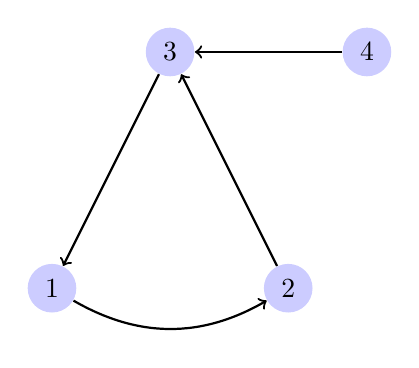
\begin{tikzpicture}

\tikzset{vertex/.style = {circle, fill =blue!20}}
\tikzset{edge/.style = {->, thick}}
%\draw[help lines] (0,0) grid (6,6);
\node[vertex] (a) at (0,1) {1};
\node[vertex] (b) at (3,1){2};
\node[vertex] (c) at (1.5,4){3};
\node[vertex] (d) at (4,4){4};

\draw[edge] (a) to[bend right] (b);
\draw[edge] (b) to (c);
\draw[edge] (c) to (a);
\draw[edge] (d) to (c);
\end{tikzpicture}
\caption{A Collision Digraph}
\end{figure}

Suppose now that $\toppre$ is found at some intermediate step in the algorithm, and consider a distinct subproblem near $\toppre$ started at $\pre_4 = (11,11,11)$ with associated isotone operator $S$.
We begin iterating and find that $S(\pre_4) = (10,10,8)$, which shows $\fix(\pre_4) \sub \fix(\toppre_3)$ 
Then a \emph{single iteration} of $S$ has shown us that $\fix(\pre_4) \sub \fix(\toppre_3) \peq (9,8,7) = \pre'$, using the relations above. 
Of course, the same conclusion would hold if we found that  $S(\pre_4) \peq \toppre_i$ for any $i$. 

We know that $\fix(\toppre_1) = \fix(\toppre_2) = \fix(\toppre_3) \peq \pre'$. 
We can track these subproblem relations efficiently with a collection of rooted trees as follows: let vertices $w_1,w_2,w_3$ be children of $w(\pre')$, a vertex representing $\pre' = (9,8,7)$. 
We denote this relationship by $c(w(\pre')) = \{w_1,w_2,w_3\}$.
Using the notation in the previous section, we have the root-vertex relation $r(w_i) = w(\pre')$ for $i = 1,2,3$. 
Note that, by our work above, we have $\fix(\pre') = \fix(\toppre_i)$ for all $w_i \in c(w(\pre'))$. 
Also, $\fix(\toppre_i) = \fix(\toppre_j)$ for all $i,j$ children of the same node. 

Suppose we maintain a collection of trees for which parent nodes and child nodes are all related in this way. 
Consider a solved subproblem $\lag \pre_i \rag$ with $r(w_i) = w_k$.
Then if at some step of the algorithm we obtain a guarantee that $\fix(\pre_j) \sub \fix(\pre_i)$ for an active subproblem $\lag \pre_j \rag$, the relations built into our problem tree imply that, in fact, $\fix(\pre_j) \sub \fix(\pre_k)$, potentially \emph{skipping a large region of lattice space} that we would otherwise have to search for elements of $\fix(T)$. 
This dynamic gives our algorithm a ``Chutes and Ladders'' effect. 
In particular, we make efficient use of both the geometric information shared between active problems and the information gained during previous steps of the algorithm. 

\begin{figure} \label{fig:forest} 
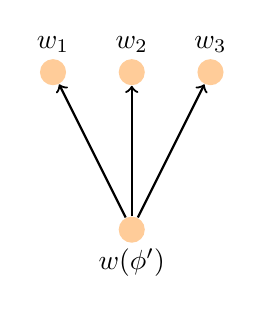
\begin{tikzpicture}
\tikzset{vertex2/.style = {circle, fill =orange!40}}
\tikzset{edge/.style = {->, thick}}

\node[vertex2] (e) at (3,1) {};
\node[vertex2] (f) at (2,3) {};
\node[vertex2] (g) at (3,3) {};
\node[vertex2] (h) at (4,3) {};

\draw[edge] (e) to (f);
\draw[edge] (e) to (g);
\draw[edge] (e) to (h);

\node[above = .12cm] at (f) {$w_1$};
\node[above = .12cm] at (g) {$w_2$};
\node[above = .12cm] at (h) {$w_3$};
\node[below = .12cm] at (e) {$w(\pre')$};

\end{tikzpicture}
\caption{A Problem Forest}
\end{figure}

\section{Algorithm and Results}
Due to space restrictions in this writing sample, we must content ourselves with the above intuition for our algorithm. 
We omit most of the rest of the paper, including the formal definition of a problem forest and collision digraph, and skip straight to our main results, giving bits of context as needed. 

Next, we give the algorithm. 
Due to space constraints in this writing sample, we omit full descriptions of the relevant subroutines.
For intuition, in ``InformationAcquire'' we solve subproblems and collect information about problem cone collisions, which we will eventually use to build a collision digraph.
In ``InformationCombine'', we build the collision digraph and use it to combine problem information with the help of the problem forest $\forest$.
Throughout what follows, we maintain global variables $\forest$, a rooted forest, and $\act$, a collection of active and previously solved problems.

\begin{algorithm} 
\caption{FindStrictCore} 
\label{alg:main}
\begin{algorithmic}[1]
\REQUIRE $\acto$
    \STATE Initialize as described above (omitted)
    \STATE Set $\fixfind = \emptyset$
    \WHILE{$\acto \not = \emptyset$} \label{alg3:while1}
        \STATE $(\acto, \coll, \fixtemp) \leftarrow InformationAcquire(\acto)$ 
        \STATE $\fixfind = \fixfind \cup \fixtemp$
        \WHILE{$\coll \not = \emptyset$} \label{alg3:while2}
            \STATE $(\acto,\coll) \leftarrow InformationCombine(\acto,\coll)$ 
        \ENDWHILE
    \ENDWHILE
\RETURN $\fixfind$
\end{algorithmic}
\end{algorithm}

%%%%%%% CONTROLS
%\newcommand{infacredi}{(i)}
%\newcommand{infacredii}{(ii)}
%\newcommand{infacbstopa}{(a)}
%\newcommand{infacbstopb}{(b)}
%\newcommand{infacstoptwi}{(i)}
%\newcommand{infacstoptwii}{(ii)}
%\newcommand{infacstoptwiii}{(iii)}
%\newcommand{infacstoptha}{(a)}
%\newcommand{infacstopthb}{(b)}
%%%%%%%

\begin{lemma} \label{lemma:key}
At any point during the execution of FindStrictCore 
\begin{enumerate}
\item $\forest$ is a problem forest \label{convlemma:forest}
\item If $k \in \coll(i)$, where $r(w_i) = w_j$, then $\fix(\pre_j) \sub \fix(\pre_k)$ \label{convlemma:coll}
\end{enumerate}
\end{lemma}
The following proposition shows that, conditional on the problem forest structure of $\forest$, the collision digraph can be used to combine the information contained in distinct problem cones.
\begin{prop} \label{prop:graph}
Suppose that the following conditions hold when InformationCombine is called: 
\begin{enumerate}
\item[(i)] $\forest$ is a problem forest
\item[(ii)] For any $\pre_i \in \acto$ with $r(w_i) = w_j$, if $k \in \coll(i)$ then $\fix(\pre_j) \sub \fix(\pre_k)$
\end{enumerate}
Let $G = (V,E)$ be the collision digraph and $S$ one of its strong components, then 
\begin{enumerate}
\item If $(v_i, v_k) \in E$ then $\fix(\pre_i) \sub \fix(\pre_k)$. \label{prop:graph:edge}
\item If $v_i, v_j \in \strongcomp$ then $\fix(\pre_i) = \fix(\pre_j)$. \label{prop:graph:strong}
\item If $v_j \in \strongcomp$ and $v_k \in \reach$, the reachable set of $\strongcomp$, then $\fix(\pre_i) \peq \pre_k$. \label{prop:graph:reach}
\end{enumerate}
\end{prop}
In particular, item~(\ref{prop:graph:strong}) shows that the strong components of $G$ identify groups of equivalent problems, which can then be consolidated.
Statement (3) shows that fast digraph algorithms for computing reachable sets can be used to combine the information learned in different subproblems.

After a series of omitted lemmas, we get the following results:

\begin{lemma} \label{lemma:termination}
FindStrictCore terminates in finite time
\end{lemma}

\begin{thm} \label{thm:correct}
FindStrictCore returns with $ \fixfind = \fix(T)$.
In particular, the algorithm finds all core outcomes $\strcore = \{Y: \pre_Y \in \fixfind \}$. 
\end{thm}

\section{Maximal Domain Results and Generalizations} 
Omitted for the purposes of this writing sample.

\section{Finding All Stable Matchings} 
In this section, we extend the information sharing technique developed above to an algorithm for finding all stable allocations in the setting of two-sided many-to-many matching with contracts under the assumption of substitutable preferences.
Here, we think of the contract language as $X = D\times H \times E$, where $E$ is a set of contract terms, $D$ is a set of doctors, and $H$ is a set of hospitals (all finite). 

We define choice functions in the usual way for $Y\in 2^{X_a}$ as 
\[
C_a(Y) = \argmax_{Z\subseteq Y} \, U_a(Z)
\]
and, with abuse of notation, extend these functions to $Y\in 2^X$ by setting $C_a(Y) \equiv C_a(Y_a)$.
For $Y \in 2^X$, we set $C_D(Y) = \bigcup_{d \in D} C_d(Y)$ and similarly for hospitals.

\subsubsection{Fixed Point Construction}
Consider a lattice $\lattice = 2^X \times 2^X$, pairs of subsets of $X$, where we define a partial order by $(Z,W) \peq (Z',W')$ if and only if $Z \sub Z'$ and $W' \sub W$. 
It is easy to check that this partial order defines a complete lattice.
For instance, given a collection of $(Z_i, W_i) \in \lattice$, the greatest lower bound is $\bigwedge_i (Z_i, W_i) = \lft \bigcap_i Z_i, \bigcup_i W_i \rt \in 2^X \times 2^X$.
The least upper bound is attained similarly by swapping unions and intersections. 

As in \cite{HatfieldKominers2010b}, we may define an operator $\Phi: \lattice \to \lattice$ by $\Phi(Z,W) = (\Phi_D(W), \Phi_H(Z))$, where $\Phi^D(Z) = \{z \in X: z \in C_D(\{z \} \cup Z) \}$ and $\Phi^H(W) = \{z \in X: z \in C_H(\{z \} \cup W) \}$.
As usual, we define the fixed point set $\fix(\Phi) \equiv \{(Z,W) \in 2^X \times 2^X: \Phi(Z,W) = (Z,W) \}$.
It is easy to see from the definition of substitutability that this operator is isotone on $\lattice$.
Therefore, by Tarski's Theorem, $\fix(\Phi)$ is a non-empty lattice.

The following characterization of stable matchings is due to \cite{HatfieldKominers2010b} 
\begin{lemma}[\cite{HatfieldKominers2010b}, Lemma 1] \label{lemma:hk}
Assume that agents' preferences are substitutable and satisfy irrelevance of rejected contracts.
Then for any $(Z,W) \in \fix(\Phi)$, we have $Z\cap W \in \stable$.
Conversely, for any $Y\in \stable$, there exists a unique $(Z,W) \in \fix(\Phi)$ such that $Z \cap W = Y$.
\end{lemma}

\subsubsection{Definition of Sublattice Operators} - This lemma shows that, for the case of substitutable preferences, finding all stable matchings $\stable$ is equivalent to finding all fixed points of the operator $\fix(\Phi)$.
By isotonicity of $\Phi$, the standard Tarski argument from previous sections shows that the sequence formed by $\Phi^k(X, \emptyset)$ is monotonically decreasing, and fixes at $(\topx, \topy) = \max \fix(\Phi)$.
Similarly, iterating $\Phi^k(\emptyset, X)$ eventually fixes at a $(\botx, \boty) = \min \fix( \Phi)$.
Note then that any $(Z,W) \in \fix(\Phi)$ (corresponding to stable allocation $Z \cap W$) satisfies $\botx \sub Z \sub \topx$ and $\topy \sub W \sub \boty$.

This observation motivates our definition of operators on sublattices of $\lattice$.
Specifically, for a fixed element $(\topx, \topy) \suq (X_i, Y_i) \suq (\botx, \boty)$, where $i$ is an index, we let $\lattice_i \equiv \{(Z,W): (Z,W) \peq (X_i, Y_i) \}$ and note that this is a complete sublattice.
Define $\Phi_i: \lattice \to \lattice$ by setting $\Phi_i(Z,W) = (\Phi^D_i(W), \Phi^H_i(Z))$, where $\Phi^D_i(W) = \{z \in X_i \setminus \botx: z \in C_H(\{z\} \cup W) \} \cup \botx$ and $\Phi^H_i(Z) = \{z \in \boty \setminus Y_i: z \in C_D( \{z \} \cup Z ) \} \cup Y_i$.

\subsection{Fixed Point Guarantees and Initializing Subproblems}

The following result shows that the family of operators introduced above satisfies the conditions required for an information sharing algorithm on the lattice $\lattice = 2^X \times 2^X$. 

\begin{lemma} \label{lemma:phigar}
Suppose that agents' preferences are substitutable over $X$.
Let the sublattice $\lattice_i$ and $\Phi_i: \lattice \to \lattice$ be defined as above for some $(X_i, Y_i) \suq (\botx, \boty)$. 
Then the following statements are true
\begin{enumerate}
\item $\Phi_i: \lattice_i \to \lattice_i$ and is isotone. 
\item$\fix(\Phi) \cap \lattice_i \sub \fix(\Phi_i)$.
\end{enumerate}
\end{lemma}

The proof of this section's main result is similar to the proof of Theorem~\ref{thm:correct} and crucially relies on Lemma~\ref{lemma:phigar} above. 

\begin{thm} \label{thm:correct2}
FindStable returns $\fixfind = \fix(\Phi)$. 
In particular, $\{Z \cap W: (Z,W) \in \fixfind\} = \stable$, so the algorithm finds all stable allocations.
\end{thm}

\section{Conclusion}
The approach developed above gives an alternative method for computing reasonable economic outcomes in general matching markets when substitutability is not guaranteed. 
Our technique has several applications to computing objects of interest in economic problems for which there is a lattice structure.
The information sharing approach developed here also gives the first algorithm for finding all stable allocations in bilateral matching with contracts with substitutable preferences.

\bibliographystyle{chicago}
\bibliography{ConeReferences}

\end{document}


